\documentclass[12pt,a4paper]{article}

% ─── Page Layout ───────────────────────────────────────────────────────────────
\usepackage[a4paper, margin=0.8in, headheight=14pt]{geometry}

% ─── Fonts (XeLaTeX) ───────────────────────────────────────────────────────────
\usepackage{fontspec}
\usepackage{unicode-math}
\setmainfont{TeX Gyre Pagella}
\setmonofont[Scale=0.88]{TeX Gyre Cursor}
\setmathfont{Latin Modern Math}

% ─── Packages ──────────────────────────────────────────────────────────────────
\usepackage{xcolor}
\usepackage{colortbl}
\usepackage{titlesec}
\usepackage{enumitem}
\usepackage{tabularx}
\usepackage{booktabs}
\usepackage{array}
\usepackage{amsmath}
\usepackage{tikz}
\usetikzlibrary{shapes.geometric, arrows.meta, positioning, calc, fit, decorations.pathreplacing}
\usepackage{tcolorbox}
\tcbuselibrary{skins, breakable}
\usepackage{hyperref}
\usepackage{fancyhdr}
\usepackage{graphicx}
\usepackage{microtype}
\hyphenpenalty=10000
\exhyphenpenalty=10000
\sloppy
\usepackage{caption}
\usepackage{setspace}
\usepackage{multirow}
\usepackage{tocloft}

% ─── Q&A helper ────────────────────────────────────────────────────────────────
\newcommand{\Q}[1]{\textbf{#1}\par\noindent\ignorespaces}

% ─── Colour Palette ────────────────────────────────────────────────────────────
\definecolor{myred}{RGB}{196,30,58}
\definecolor{mydark}{RGB}{30,30,50}
\definecolor{mygreen}{RGB}{14,120,80}
\definecolor{myteal}{RGB}{0,130,140}
\definecolor{myamber}{RGB}{180,100,0}
\definecolor{mypurple}{RGB}{100,30,160}
\definecolor{mygray}{RGB}{246,247,249}
\definecolor{mgframe}{RGB}{180,185,200}
\definecolor{watermark}{RGB}{145,150,170}
\definecolor{hdrred}{RGB}{250,232,235}
\definecolor{hdrgreen}{RGB}{220,244,233}
\definecolor{hdrteal}{RGB}{220,242,244}
\definecolor{hdramber}{RGB}{253,242,215}
\definecolor{hdrpurple}{RGB}{238,228,255}
\definecolor{hdrgray}{RGB}{238,240,245}
\definecolor{rowalt}{RGB}{250,251,253}

% ─── Section Formatting ────────────────────────────────────────────────────────
\titleformat{\section}
  {\large\bfseries\color{myred}}{\thesection.}{0.5em}{}
  [\vspace{1pt}{\color{myred}\rule{\linewidth}{0.8pt}}]
\titleformat{\subsection}
  {\normalsize\bfseries\color{myteal}}{\thesubsection}{0.5em}{}
\titlespacing*{\section}{0pt}{18pt}{7pt}
\titlespacing*{\subsection}{0pt}{11pt}{4pt}

% ─── Paragraph ─────────────────────────────────────────────────────────────────
\setlength{\parindent}{0pt}
\setlength{\parskip}{4pt}

% ─── TOC Styling ───────────────────────────────────────────────────────────────
\renewcommand{\cfttoctitlefont}{\large\bfseries\color{myred}}
\renewcommand{\cftaftertoctitle}{\par\noindent{\color{myred}\rule{\linewidth}{0.8pt}}}
\setlength{\cftbeforetoctitleskip}{0pt}
\setlength{\cftaftertoctitleskip}{6pt}
\renewcommand{\cftsecfont}{\normalsize\bfseries\color{mydark}}
\renewcommand{\cftsecpagefont}{\normalsize\bfseries\color{mydark}}
\renewcommand{\cftsecleader}{\cftdotfill{\cftdotsep}}
\setlength{\cftbeforesecskip}{7pt}
\renewcommand{\cftsubsecfont}{\small\color{mydark}}
\renewcommand{\cftsubsecpagefont}{\small\color{mydark}}
\setlength{\cftbeforesubsecskip}{3pt}
\setlength{\cftsubsecindent}{1.4em}

% ─── Table helpers ─────────────────────────────────────────────────────────────
\renewcommand{\arraystretch}{1.45}
\setlength{\tabcolsep}{6pt}
\arrayrulecolor{mydark}
\newcolumntype{B}[1]{>{\small\bfseries\raggedright\arraybackslash}m{#1}}
\newcolumntype{Y}{>{\small\raggedright\arraybackslash}X}
\renewcommand{\tabularxcolumn}[1]{m{#1}}

% ─── Header / Footer ───────────────────────────────────────────────────────────
\pagestyle{fancy}
\fancyhf{}
\fancyhead[L]{\small\color{myred}\textbf{PE-EC702A}\;\color{mydark}--- Adaptive Signal Processing}
\fancyhead[R]{\small\color{myteal}\textbf{Module 3 Notes}}
\fancyfoot[C]{\small\color{mydark}\thepage}
\fancyfoot[R]{\small\color{watermark}\textit{\copyright\ Biraj}}
\renewcommand{\headrulewidth}{0.5pt}
\renewcommand{\footrulewidth}{0.3pt}

% ─── Hyperref ──────────────────────────────────────────────────────────────────
\hypersetup{
  colorlinks=true, linkcolor=myteal, urlcolor=myteal,
  pdfauthor={Biraj Sarkar},
  pdftitle={PE-EC702A --- Module 3 Notes}
}

% ─── tcolorbox styles ──────────────────────────────────────────────────────────
\tcbset{
  tikzbox/.style={
    colback=mygray, colframe=mgframe, boxrule=0.6pt, arc=4pt,
    left=8pt, right=8pt, top=6pt, bottom=6pt,
    colbacktitle=mgframe, coltitle=mydark,
    fonttitle=\small\bfseries
  },
  defbox/.style={
    colback=hdrgreen, colframe=mygreen, boxrule=0.8pt, arc=4pt,
    left=9pt, right=9pt, top=6pt, bottom=6pt,
    colbacktitle=mygreen, coltitle=white,
    fonttitle=\small\bfseries
  },
  formulabox/.style={
    colback=hdrteal, colframe=myteal, boxrule=0.8pt, arc=4pt,
    left=9pt, right=9pt, top=7pt, bottom=7pt,
    colbacktitle=myteal, coltitle=white,
    fonttitle=\small\bfseries
  },
  examplebox/.style={
    colback=hdramber, colframe=myamber, boxrule=0.8pt, arc=4pt,
    left=9pt, right=9pt, top=6pt, bottom=6pt,
    colbacktitle=myamber, coltitle=white,
    fonttitle=\small\bfseries
  },
  masonbox/.style={
    colback=hdrpurple, colframe=mypurple, boxrule=0.8pt, arc=4pt,
    left=9pt, right=9pt, top=6pt, bottom=6pt,
    colbacktitle=mypurple, coltitle=white,
    fonttitle=\small\bfseries
  },
  exambox/.style={
    colback=hdrpurple, colframe=mypurple, boxrule=1pt, arc=5pt,
    left=10pt, right=10pt, top=8pt, bottom=8pt,
    colbacktitle=mypurple, coltitle=white,
    fonttitle=\bfseries,
    breakable, title after break={\textbf{Frequently Asked / Viva Questions (contd.)}}}
}
\tcbset{breakable}

% ─── TikZ styles ───────────────────────────────────────────────────────────────
\tikzset{
  block/.style={rectangle, draw=myteal, fill=hdrteal,
    text width=2.4cm, align=center, minimum height=0.95cm,
    font=\small, rounded corners=3pt, line width=0.7pt},
  redblock/.style={rectangle, draw=myred, fill=hdrred,
    text width=2.4cm, align=center, minimum height=0.95cm,
    font=\small, rounded corners=3pt, line width=0.7pt},
  netnode/.style={rectangle, draw=myteal, fill=hdrteal,
    text width=1.5cm, align=center, minimum height=0.8cm,
    font=\small, rounded corners=3pt, line width=0.7pt},
  sumjunc/.style={circle, draw=myamber, fill=hdramber,
    minimum size=0.62cm, font=\small, line width=0.8pt},
  snode/.style={circle, draw=mypurple, fill=hdrpurple,
    minimum size=0.55cm, font=\footnotesize, line width=0.7pt},
  arrow/.style={-Stealth, thick, color=mydark},
  redarrow/.style={-Stealth, thick, color=myred},
  line/.style={thick, color=mydark}
}

% ═══════════════════════════════════════════════════════════════════════════════
\begin{document}
% ═══════════════════════════════════════════════════════════════════════════════

\begin{center}
  {\LARGE\bfseries\color{myred} PE-EC702A --- Adaptive Signal Processing}\\[5pt]
  {\normalsize\color{mydark} Semester VII \quad$\bullet$\quad 3L:0T:0P \quad$\bullet$\quad 3 Credits}\\[3pt]
  {\normalsize\color{myteal}\textbf{Module 3 Exam Notes: LMS Variants \& Signal Space Concepts}}\\[3pt]
  {\small\color{mydark} CGEC \;$|$\; B.Tech ECE (2023--27) \;$|$\; \textit{Biraj Sarkar}}
\end{center}
\vspace{2pt}
\noindent{\color{myred}\rule{\linewidth}{1.5pt}}
\vspace{2pt}

\hypersetup{linkcolor=mydark}
\tableofcontents
\hypersetup{linkcolor=myteal}
\newpage

% ===============================================================================
\section{Variants of the LMS Algorithm}
% ===============================================================================

To overcome constraints of standard LMS (computational complexity, time-varying power instability, or convergence rates), several variants are employed.

\subsection{The Sign-LMS Family}
Designed to reduce computational requirements in high-speed hardware by replacing multiplications with sign operations. The vector sign function $\text{sgn}(\cdot)$ extracts element-wise signs ($\pm 1$ or $0$).
\begin{enumerate}[label=\textbf{\arabic*.}, leftmargin=*, itemsep=3pt]
  \item \textbf{Sign-Error LMS:} Simplifies the error term.
  \begin{equation}
    \mathbf{w}(n+1) = \mathbf{w}(n) + \mu \operatorname{sgn}(e(n)) \mathbf{x}(n)
  \end{equation}
  \item \textbf{Sign-Data (Regressor) LMS:} Simplifies the regressor data vector.
  \begin{equation}
    \mathbf{w}(n+1) = \mathbf{w}(n) + \mu e(n) \operatorname{sgn}(\mathbf{x}(n))
  \end{equation}
  \item \textbf{Sign-Sign LMS:} Simplifies both terms; updates require only additions (no multiplications).
  \begin{equation}
    \mathbf{w}(n+1) = \mathbf{w}(n) + \mu \operatorname{sgn}(e(n)) \operatorname{sgn}(\mathbf{x}(n))
  \end{equation}
\end{enumerate}

\subsection{Normalized LMS (NLMS) Algorithm}
In standard LMS, the step-size is bounded by the signal power ($0 < \mu < 2/\text{Tr}(\mathbf{R})$). If the input power varies widely (like speech), standard LMS can diverge during high-power segments. NLMS solves this by normalizing the step-size with the instantaneous squared norm of the input vector:
\begin{equation}
  \mathbf{w}(n+1) = \mathbf{w}(n) + \frac{\tilde{\mu}}{\|\mathbf{x}(n)\|^2 + \epsilon} e^*(n) \mathbf{x}(n)
\end{equation}
where $\tilde{\mu}$ is the normalized step-size ($0 < \tilde{\mu} < 2$), and $\epsilon > 0$ is a small regularization parameter preventing division by zero.

\subsection{Block LMS (BLMS) and FFT-Based Realizations}
Standard LMS updates weights sample-by-sample. Block LMS updates the weights only once per block of $L$ input samples, averaging the gradients over the block:
\begin{equation}
  \mathbf{w}(k+1) = \mathbf{w}(k) + \frac{2\mu}{L} \sum_{i=0}^{L-1} e(kL + i) \mathbf{x}(kL + i)
\end{equation}
where $k$ is the block index.
\begin{itemize}[leftmargin=*, itemsep=2pt]
  \item \textbf{FFT Realization (FDAF):} Block convolution and correlation can be computed in the frequency domain using Fast Fourier Transforms (FFTs) via the overlap-save or overlap-add method. This reduces computational complexity from $O(M^2)$ to $O(M \log_2 M)$ for large tap lengths.
\end{itemize}

\subsection{Sub-band Adaptive Filtering}
In sub-band adaptive filters, the wideband input and desired signals are split into $N$ sub-bands using an analysis filter bank. Adaptive filtering is performed on each sub-band signal after decimation (downsampling). Finally, a synthesis filter bank reconstructs the full-band output.
\begin{itemize}[leftmargin=*, itemsep=2pt]
  \item \textbf{Advantages:} Decimation reduces the operating sampling rate. Sub-band signals have a much whiter spectral envelope (smaller eigenvalue spread) than the original wideband signal, significantly accelerating convergence.
\end{itemize}

% ===============================================================================
\section{Signal Space Concepts}
% ===============================================================================

To formulate advanced algorithms like RLS, signals are viewed as elements of abstract vector spaces (Hilbert spaces).

\subsection{Vector Space and Subspace Theory}
A vector space $V$ over a field $F$ (typically complex numbers $\mathbb{C}$) is a set of elements closed under vector addition and scalar multiplication, satisfying the standard vector space axioms.
\begin{itemize}[leftmargin=*, itemsep=3pt]
  \item \textbf{Subspace:} A subset $W \subseteq V$ is a subspace if it is closed under vector addition and scalar multiplication.
  \item \textbf{Basis and Dimension:} A set of vectors $\{v_1, \dots, v_k\}$ forms a basis for $V$ if they are linearly independent and span $V$. The number of vectors in the basis is the dimension $\dim(V)$.
  \item \textbf{Linear Operators, Rank and Nullity:} For a linear operator $T: V \to W$, the range space is $\mathcal{R}(T)$ and null space is $\mathcal{N}(T)$. The dimensions are rank $\rho(T) = \dim(\mathcal{R}(T))$ and nullity $\nu(T) = \dim(\mathcal{N}(T))$. The Rank-Nullity Theorem states:
  \begin{equation}
    \rho(T) + \nu(T) = \dim(V)
  \end{equation}
\end{itemize}

\subsection{Inner Product Space and Orthogonality}
An inner product space is a vector space $V$ equipped with an inner product $\langle u, v \rangle$, mapping two vectors to a scalar, satisfying conjugate symmetry ($\langle u,v \rangle = \langle v,u \rangle^*$), linearity, and positive definiteness ($\langle u,u \rangle \ge 0$).
\begin{itemize}[leftmargin=*, itemsep=2pt]
  \item \textbf{Induced Norm:} $\|u\| = \sqrt{\langle u, u \rangle}$.
  \item \textbf{Orthogonality:} Two vectors are orthogonal if $\langle u, v \rangle = 0$.
  \item \textbf{Orthogonal Decomposition:} Any vector space $V$ with a closed subspace $W$ can be decomposed uniquely as:
  \begin{equation}
    V = W \oplus W^\perp
  \end{equation}
  where $W^\perp = \{v \in V \mid \langle v, w \rangle = 0 \; \forall w \in W\}$ is the orthogonal complement.
\end{itemize}

\subsection{Gram-Schmidt Orthogonalization}
A recursive algorithm that converts a set of linearly independent vectors $\{v_1, v_2, \dots, v_M\}$ into an orthonormal set $\{q_1, q_2, \dots, q_M\}$ spanning the same space:
\begin{align}
  u_1 &= v_1, \quad q_1 = \frac{u_1}{\|u_1\|} \nonumber \\
  u_k &= v_k - \sum_{j=1}^{k-1} \langle v_k, q_j \rangle q_j, \quad q_k = \frac{u_k}{\|u_k\|} \quad \text{for } k=2, \dots, M
\end{align}

\subsection{Orthogonal Projection}
The orthogonal projection of a vector $x$ onto a subspace $W$ spanned by orthonormal vectors $\{q_1, \dots, q_k\}$ is:
\begin{equation}
  P_W(x) = \sum_{i=1}^k \langle x, q_i \rangle q_i
\end{equation}
The projection error $e = x - P_W(x)$ is orthogonal to the subspace $W$ ($\langle e, w \rangle = 0 \; \forall w \in W$), which is the geometric basis of the Orthogonality Principle.

\begin{tcolorbox}[tikzbox, title={Vector Projection Geometry}]
\centering
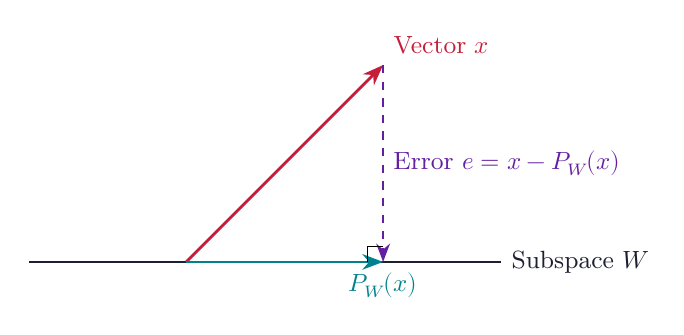
\begin{tikzpicture}[every node/.style={font=\small}]
  % Subspace W (horizontal plane represented by a line)
  \draw[thick, color=mydark] (-2,0) -- (4,0) node[right] {Subspace $W$};
  
  % Vector x (pointing up-right)
  \draw[arrow, color=myred, line width=1pt] (0,0) -- (2.5,2.5) node[above right] {Vector $x$};
  
  % Projection P_W(x)
  \draw[arrow, color=myteal, line width=1pt] (0,0) -- (2.5,0) node[below] {$P_W(x)$};
  
  % Error vector e (vertical dashed arrow)
  \draw[arrow, dashed, color=mypurple, line width=0.8pt] (2.5,2.5) -- (2.5,0) node[midway, right] {Error $e = x - P_W(x)$};
  
  % Orthogonality square indicator
  \draw (2.5,0.2) -- (2.3,0.2) -- (2.3,0);
\end{tikzpicture}
\end{tcolorbox}

\begin{tcolorbox}[examplebox, title={Example: Gram-Schmidt Orthonormalization}]
Apply the Gram-Schmidt process to the following set of vectors in $\mathbb{R}^3$ to obtain an orthonormal basis:
\[
  v_1 = [1, 1, 0]^T, \quad v_2 = [1, 2, 0]^T, \quad v_3 = [0, 1, 2]^T
\]

\textbf{Solution:}
\begin{enumerate}[label=\textbf{\arabic*.}, leftmargin=*, itemsep=4pt]
  \item For $v_1$:
    \[
      u_1 = v_1 = [1, 1, 0]^T \implies \|u_1\| = \sqrt{1^2 + 1^2 + 0^2} = \sqrt{2}
    \]
    \[
      q_1 = \frac{u_1}{\|u_1\|} = \left[\frac{1}{\sqrt{2}}, \frac{1}{\sqrt{2}}, 0\right]^T
    \]
  \item For $v_2$:
    \[
      \langle v_2, q_1 \rangle = (1 \times \frac{1}{\sqrt{2}}) + (2 \times \frac{1}{\sqrt{2}}) + 0 = \frac{3}{\sqrt{2}}
    \]
    \[
      u_2 = v_2 - \langle v_2, q_1 \rangle q_1 = \begin{bmatrix} 1 \\ 2 \\ 0 \end{bmatrix} - \frac{3}{\sqrt{2}}\begin{bmatrix} 1/\sqrt{2} \\ 1/\sqrt{2} \\ 0 \end{bmatrix} = \begin{bmatrix} 1 \\ 2 \\ 0 \end{bmatrix} - \begin{bmatrix} 1.5 \\ 1.5 \\ 0 \end{bmatrix} = \begin{bmatrix} -0.5 \\ 0.5 \\ 0 \end{bmatrix}
    \]
    \[
      \|u_2\| = \sqrt{(-0.5)^2 + 0.5^2 + 0} = \sqrt{0.5} = \frac{1}{\sqrt{2}}
    \]
    \[
      q_2 = \frac{u_2}{\|u_2\|} = \sqrt{2} \begin{bmatrix} -0.5 \\ 0.5 \\ 0 \end{bmatrix} = \left[-\frac{1}{\sqrt{2}}, \frac{1}{\sqrt{2}}, 0\right]^T
    \]
  \item For $v_3$:
    \[
      \langle v_3, q_1 \rangle = \frac{1}{\sqrt{2}}, \quad \langle v_3, q_2 \rangle = \frac{1}{\sqrt{2}}
    \]
    \[
      u_3 = v_3 - \langle v_3, q_1 \rangle q_1 - \langle v_3, q_2 \rangle q_2 = \begin{bmatrix} 0 \\ 1 \\ 2 \end{bmatrix} - \frac{1}{2}\begin{bmatrix} 1 \\ 1 \\ 0 \end{bmatrix} - \frac{1}{2}\begin{bmatrix} -1 \\ 1 \\ 0 \end{bmatrix} = \begin{bmatrix} 0 \\ 0 \\ 2 \end{bmatrix}
    \]
    \[
      \|u_3\| = 2 \implies q_3 = \frac{u_3}{\|u_3\|} = [0, 0, 1]^T
    \]
\end{enumerate}
The orthonormal basis is:
\[
  \left\{ \begin{bmatrix} 1/\sqrt{2} \\ 1/\sqrt{2} \\ 0 \end{bmatrix}, \begin{bmatrix} -1/\sqrt{2} \\ 1/\sqrt{2} \\ 0 \end{bmatrix}, \begin{bmatrix} 0 \\ 0 \\ 1 \end{bmatrix} \right\}
\]
\end{tcolorbox}

% ===============================================================================
% MANDATORY QUICK REVISION PAGE
% ===============================================================================
\newpage
\begin{center}
  {\large\bfseries\color{myred} Quick Revision --- Module III}\\[3pt]
  {\small\color{mydark} LMS Variants \& Signal Space Concepts $|$ PE-EC702A}
\end{center}
\noindent{\color{myred}\rule{\linewidth}{1.2pt}}
\vspace{4pt}

\begin{tcolorbox}[formulabox, title={\textbf{Key Formulas at a Glance}}]
\renewcommand{\arraystretch}{1.3}
\begin{tabularx}{\linewidth}{B{4.5cm} X}Sign-Error LMS & $\mathbf{w}(n+1) = \mathbf{w}(n) + \mu \operatorname{sgn}(e(n)) \mathbf{x}(n)$ \\[6pt]
Sign-Sign LMS & $\mathbf{w}(n+1) = \mathbf{w}(n) + \mu \operatorname{sgn}(e(n)) \operatorname{sgn}(\mathbf{x}(n))$ \\[6pt]
Normalized LMS Update & $\mathbf{w}(n+1) = \mathbf{w}(n) + \frac{\tilde{\mu}}{\|\mathbf{x}(n)\|^2 + \epsilon} e^*(n) \mathbf{x}(n)$ \\[6pt]
Rank-Nullity Theorem & $\text{rank}(T) + \text{nullity}(T) = \dim(V)$ \\[6pt]
Orthogonal Projection & $P_W(x) = \sum_{i=1}^k \langle x, q_i \rangle q_i$ \quad ($q_i$: orthonormal basis) \\[6pt]
Gram-Schmidt Step & $u_k = v_k - \sum_{j=1}^{k-1} \langle v_k, q_j \rangle q_j, \quad q_k = u_k/\|u_k\|$
\end{tabularx}
\end{tcolorbox}

\begin{tcolorbox}[defbox, title={\textbf{One-Line Definitions}}]
\begin{itemize}[leftmargin=*, itemsep=2.5pt, topsep=0pt]
  \item \textbf{Normalized LMS:} A variant of LMS that divides step-size by input power to maintain stability.
  \item \textbf{Sign-Sign LMS:} A hardware-friendly LMS variant using only signs of data and error.
  \item \textbf{Inner Product Space:} A vector space equipped with a function defining angles and lengths (norms).
  \item \textbf{Gram-Schmidt Process:} An algorithm generating orthonormal bases from a set of linearly independent vectors.
  \item \textbf{Rank of Operator:} The dimension of the range space of a linear transformation.
  \item \textbf{Nullity of Operator:} The dimension of the null space of a linear transformation.
\end{itemize}
\end{tcolorbox}

\begin{tcolorbox}[exambox, title={\textbf{Frequently Asked / Viva Questions}}]
\begin{enumerate}[topsep=0pt, label=\textbf{Q\arabic*.}, itemsep=5pt]
  \item \Q{What is the primary advantage of Sign-LMS algorithms?}
    They reduce hardware multiplier requirements. Sign-Sign LMS replaces the update multiplications with simple addition/subtraction, accelerating hardware processing.
  \item \Q{Why does standard LMS sometimes diverge with speech inputs and how does NLMS solve it?}
    Speech has highly variable power. During high-amplitude segments, the fixed step-size of standard LMS can violate bounds ($2/\text{Tr}(\mathbf{R})$), causing divergence. NLMS scales $\mu$ inversely with instantaneous power, ensuring stability.
  \item \Q{State the Rank-Nullity Theorem.}
    For any linear operator $T: V \to W$ where $V$ is finite-dimensional, $\dim(\mathcal{R}(T)) + \dim(\mathcal{N}(T)) = \dim(V)$, meaning Rank + Nullity = Dimension of domain.
  \item \Q{Explain overlap-save block processing in FDAF.}
    It is a frequency-domain technique that computes block convolutions of input signals with filter weights using DFTs/FFTs, avoiding time-domain convolution overhead.
  \item \Q{What is sub-band adaptive filtering and why is it used?}
    It divides a wideband signal into multiple narrower frequency bands. It speeds up convergence by reducing the eigenvalue spread (whitening) and lowers computational complexity by decimation.
  \item \Q{Define the orthogonal complement of a subspace.}
    The orthogonal complement $W^\perp$ of a subspace $W$ is the set of all vectors in the vector space that are orthogonal to every vector in $W$.
  \item \Q{Write the formula for the orthogonal projection of vector $x$ onto vector $y$.}
    $P_y(x) = \frac{\langle x, y \rangle}{\|y\|^2} y$.
  \item \Q{What represents the inner product of two signals $x(n)$ and $y(n)$ in $L_2$ space?}
    $\langle x, y \rangle = \sum_{n=-\infty}^\infty x(n) y^*(n)$ (for discrete signals) or $\int x(t) y^*(t) dt$ (for continuous signals).
  \item \Q{What is the regularization parameter $\epsilon$ in NLMS?}
    It is a small positive constant added to the denominator to prevent division by zero (or numerical instability) when the input vector norm $\|\mathbf{x}(n)\|$ is zero or very small.
  \item \Q{How does the computational complexity of FDAF scale with filter length $M$?}
    It scales as $O(M \log_2 M)$ compared to $O(M^2)$ for standard time-domain LMS.
\end{enumerate}
\end{tcolorbox}

\end{document}
